\documentclass{article}

\usepackage[margin = 1in]{geometry}

\usepackage{graphicx, amsmath}
\graphicspath{ {./images/} }

\title{Ch. 7 Non-Textbook Questions}
\author{Principles of Microeconomics}
\date{\today}

\begin{document}

\maketitle

\begin{enumerate}

\item Consider a market where supply is given by $Q_S = 10P - 40$ and demand is given by $Q_D = 200 - 10P$.

	\begin{enumerate}
	
	\item What is the market equilibrium price and quantity?
	
	\item What is consumer surplus at the market equilibrium?
	
	\item What is producer surplus at the market equilibrium?
	
	\item If the government implements a price floor of \$15, what quantity of the good gets traded?
	
	\item In the world of the price floor, what are consumer surplus and producer surplus?
	
	\item In the world of the price floor, what is deadweight loss?
	
	\item If the government instead implements a price ceiling of \$9, what quantity of the good gets traded?
	
	\item In the world of the price ceiling, what are consumer surplus and producer surplus?
	
	\item In the world of the price ceiling, what is deadweight loss?
	
	\item If the government instead implements a tax of \$4 per good sold on suppliers, what price do consumers end up paying?
	
	\item In the world of the tax, what price do suppliers end up receiving
	
	\item In the world of the tax, what quantity of the good gets traded?
	
	\item In the world of the tax, what are consumer surplus, producer surplus, and tax revenue?
	
	\item In the world of the tax, what is deadweight loss?
	
	\end{enumerate}
	
(Flip Page)
	
\newpage
	
\item The U.S. Department of Agriculture (USDA) administers a price floor for butter which the 2008 Farm Bill set at \$2.05 per pound. At that price, the quantity of butter supplied in 2010 was 1.7 billion pounds. The quantity demanded was 1.6 billion pounds. To support dairy farmers, the USDA chose to buy up the 100 million pound surplus. The accompanying diagram illustrates the market for butter in 2010.

	\begin{center}
	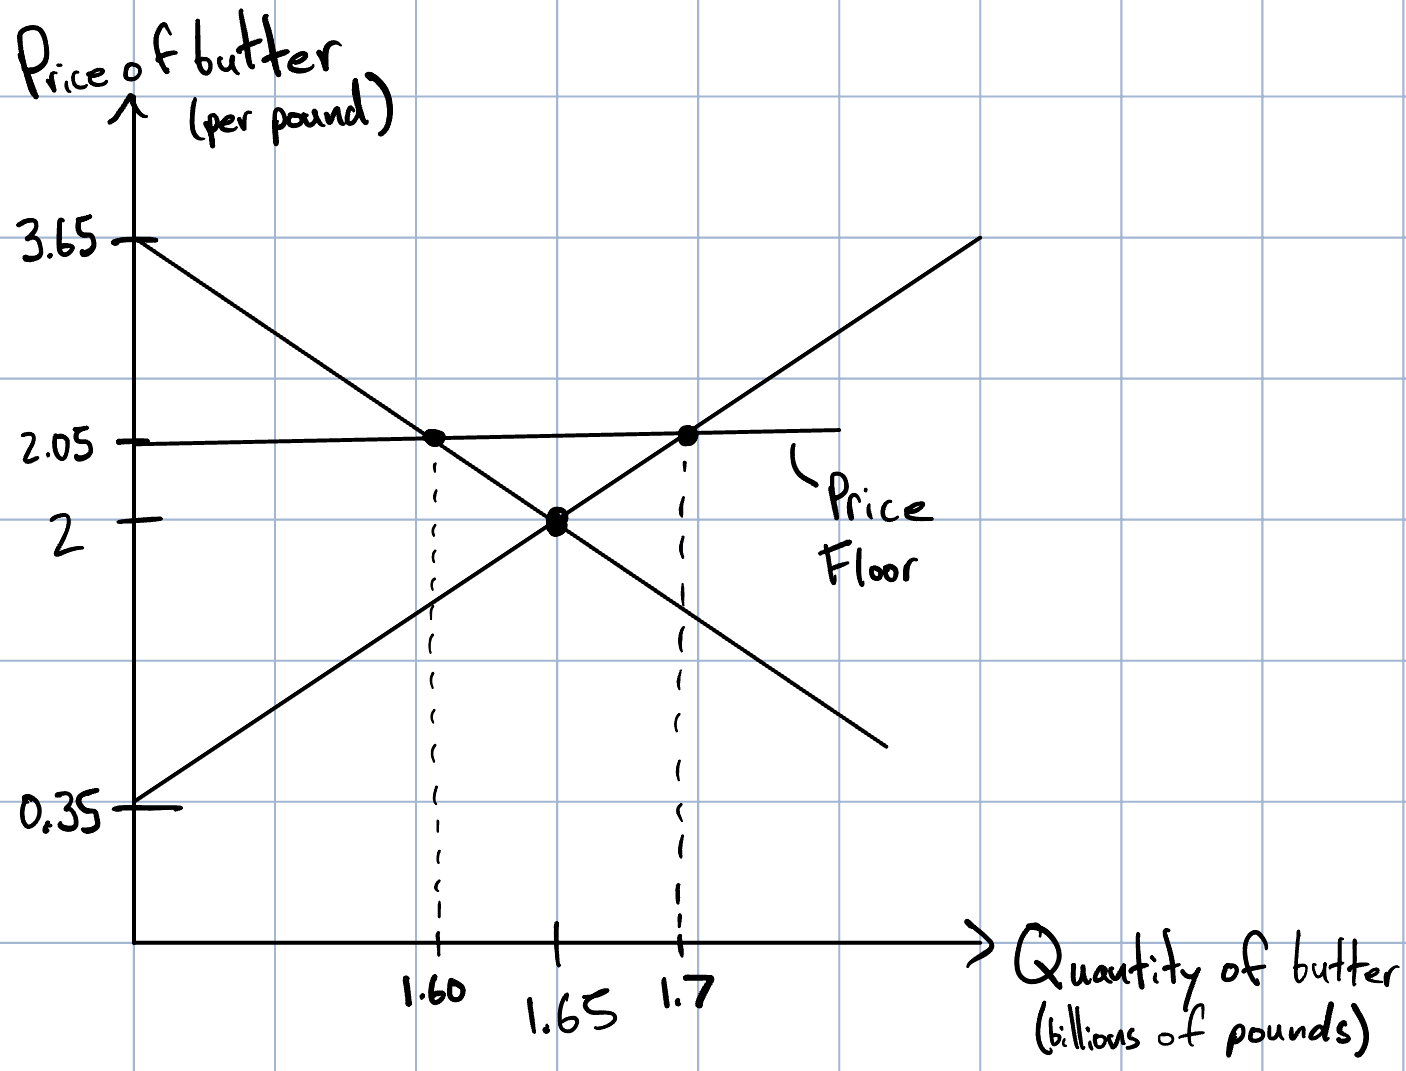
\includegraphics[width = 0.5\textwidth]{ch7_ntq2}
	\end{center}

	\begin{enumerate}
	
	\item In the absence of a price floor, how much consumer surplus would there have been? How much producer surplus? What would total surplus have been?
	
	\item What was consumer surplus with the price floor?
	
	\item What was producer surplus with the price floor? Recall that producers sold 1.7 billion pounds of butter -- some to consumers and some to the USDA.
	
	\item How much money did the USDA spend buying up surplus butter?
	
	\item The USDA had to spend tax revenue to buy up the surplus butter. Therefore, to calculate total surplus for the market, we have to subtract the decrease in tax revenue. Using your answers from parts (b)-(d), what was total surplus in the market for butter? How does this compare to total surplus without a price floor?
	
	\end{enumerate}

\end{enumerate}

\end{document}